\chapter{Electrostatics}
\section{The Electric Force}\label{sec:claw}\hypertarget{coulomb}
The attractive forces holding particles together is the \textit{electric force}. It is defined by \textbf{Coulomb's Law}:
\begin{eq}{Coulomb's Law}{1.1}\label{coulomb}
For two particles with charge $q_1$ and $q_2$ (in Coulombs) a distance $r_{12}$ from each other:
	\[
		\mathbf{F} = k \frac{q_1 q_2}{r_{12}^{2}} \hat{\mathbf{r}} 
	\] 	
\end{eq}
Where $k$ is a natural constant
\[
	k = 8.988\times 10^{9}  \mathrm{N} \cdot \frac{\mathrm{m} ^{2}}{\mathrm{C} ^{2}}
\] 
so that the force units are in Newtons. Keep in mind that $k$ may also be written (and is often done so) in the form
\[
k = \frac{1}{4\pi \epsilon_0}
\] 
where $\epsilon_0$ is another natural constant called the \textit{permittivity of free space}\footnotemark \footnotetext{Note that this should have the inverse units of $k$}:
\[
\epsilon_0 = 8.854\times 10^{-12}
\] 
Note that Equation (\ref{coulomb}) is inversely proportional to distance squared. In physics, this is known as a \textit{inverse square law} and has some important implications beyond the scope of this course.\\
It is also important to note the presence of the $\hat{\mathbf{r} }$ vector in Eq. (\ref{coulomb}). This serves to indicate that the force is oriented along the two charges, as seen below:
\begin{figure}[H]\label{clfig}
	\centering
	\scalebox{1.3}{\begin{tikzpicture}
	%\draw[lightgray] (-2,-2) grid (2,2);
	\coordinate (A) at (-1,-1);
	\coordinate (B) at (1,1);
	\coordinate (C) at (0,-1);
	\coordinate (D) at (1,-1);
	\draw[->] (A) -- (-1,2) node[left]{$y$};
	\draw[->] (A) -- (2,-1) node[right]{$x$};
	\node[anchor=south west] at (C){$\phi$};
	\draw (C) arc (0:45:1);
	\draw[dashed] (A) -- (B) node[midway,above]{$r$};
	\draw[->] (A) -- (-2,-2) node[below,left]{$\mathbf{F}_{21}$};
	\draw[->] (B) -- (2,2) node[above,right]{$\mathbf{F}_{12} $};
	\fill[white] (B) circle (0.2cm);
	\fill[white] (A) circle (0.2cm);
	\draw (B) circle (0.2cm) node[]{$+$};
	\draw (1.5,1) node[]{$q_2$};
	\draw (A) circle (0.2cm) node[]{$+$};

	\draw (-1.5,-1) node[]{$q_1$};

	\end{tikzpicture}
}
	\caption{Forces on two positively charged particles}
\end{figure}
Notice that the force of particle $q_1$ \textit{on} particle $q_2$, i.e. $\mathbf{F}_{12}$ points along the $r$ direction in the positive $x$ and $y$-axis, since both $q_1$ and $q_2$ are positive. \\[3mm]
Experimentally we have determined that Coulomb's Law obeys the \textit{principle of superposition} which states that the resultant force for a charge in a system of $n$ charges can be expressed as the vector sum of all individual forces:
\[
	\mathbf{F} _\mathrm{R} = \sum_{i=1}^n \mathbf{F}_i = \mathbf{F} _1 + \mathbf{F} _2 + \cdots + \mathbf{F} _n 
\] 
Referring back to Figure \ref{clfig}, for a vector sum it would be helpful to decompose the vectors in their basis component forms:
\[
	\mathbf{F} _{12} = F_{12}\cos \phi\; \ihat + F_{12}\sin\phi\;\jhat = \left\langle F_{12}\cos\phi,F_{12}\sin\phi \right\rangle 
\] 
This idea of vector decomposition is \textit{very} important and facilitates many important force calculations for particular arrangements of charged particles.
\section{The Electric Field}\label{sec:ef}
It's often more effective to define the electric force in the form of a vector field, where each point is defined by the electric force $\mathbf{F} $ exerted upon a test charge $q_0$ (usually positive).
\begin{eq}{Electric Field}{1.2}\label{ef}
\[
\mathbf{E} = \frac{\mathbf{F} }{q_0}
\] 	
\end{eq}
Then we can plot a direction for $\mathbf{E} $ (dependent on $\mathbf{F} $) at each point in space as seen below:
\begin{figure}[H]\label{efield1}
	\centering
	\scalebox{1.5}{
		\begin{tikzpicture}
	\coordinate (A) at (0,0);
	\coordinate (B) at (1,1);
	\coordinate (C) at (0,-1);
	\filldraw[black] (B) circle (1pt) node[above]{$q_0$};
	\filldraw[black] (C) circle (1pt) node[below]{$q_0$};
	\draw[->] (B) -- (0.5,0.5);
	\draw[->] (C) -- (0,-0.5);
	\fill[white] (A) circle (0.2cm);
	\draw (A) circle (0.2cm) node[]{$-$};	
\end{tikzpicture}

	}
	\caption{Visualizing the electric field for a negative charge}
\end{figure}
Doing this for every point in space, we get what are called \textit{field lines} for a particle. Note that these should never cross and either extend to infinity or converge at a negative particle (a \textit{sink}, perhaps?\footnotemark \footnotetext{The interested reader is encouraged to look into the differential form of Maxwell's Equations and how they relate to vector spaces.}). 

%\begin{tikzpicture}
	[decoration={markings,
	mark= at position 0.5 with {\arrow{>}}}
	]
	%\draw[lightgray] (0,0) grid (4,2);
	\coordinate (A) at (1,1);
	\coordinate (B) at (3,1);
	\draw [->-] (A) arc (180:0:1);
	%\draw[postaction={decorate}] (A) arc (120:60:2);
	\draw[->-] (A) arc (180:0:1 and 0.5);
	\draw[->-] (A) -- (B);
	\draw[postaction={decorate}] (A) arc (180:360:1 and 0.5);
	\draw[postaction={decorate}] (A) arc (180:360:1);
	%\draw[lightgray] (2,1) circle (1);
	\draw[postaction={decorate}] (A) -- (0,1);
	\draw[postaction={decorate}] (A) -- (0.2,1.8);
	\draw[postaction={decorate}] (A) -- (0.2,0.2);
	\draw[postaction={decorate}] (3.8,1.8) -- (B);
	\draw[postaction={decorate}] (4,1) -- (B);
	\draw[postaction={decorate}] (3.8,0.2) -- (B);
	\fill[white] (A) circle (0.2cm);
	\fill[white] (B) circle (0.2cm);
	\draw(A) circle (0.2cm) node[]{$+$};
	\draw (B) circle (0.2cm) node[]{$-$};
\end{tikzpicture}


\begin{figure}[H]
	\centering
	\scalebox{1.6}{
	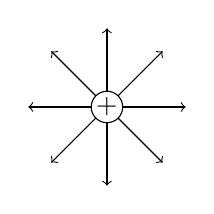
\begin{tikzpicture}
	%\draw[lightgray] (-2,-2) grid (2,2);
	\coordinate (A) at (0,0);
	%\draw (0,0) circle (1); 
	\draw[->] (A) -- (0.707,0.707);
	\draw [->] (A) -- (0,1);
	\draw[->] (A) -- (-0.707,0.707);
	\draw[->] (A) -- (-1,0);
	\draw[->] (A) -- (-0.707,-0.707);
	\draw[->] (A) -- (0,-1);
	\draw[->] (A) -- (0.707,-0.707);
	\draw[->] (A) -- (1,0);
	\fill[white] (A) circle (0.2cm);
	\draw (A) circle (0.2cm) node[]{$+$};
\end{tikzpicture}
}
	\vrule
	\scalebox{1.5}{
	\begin{tikzpicture}
	[decoration={markings,
	mark= at position 0.5 with {\arrow{>}}}
	]
	%\draw[lightgray] (0,0) grid (4,2);
	\coordinate (A) at (1,1);
	\coordinate (B) at (3,1);
	\draw [->-] (A) arc (180:0:1);
	%\draw[postaction={decorate}] (A) arc (120:60:2);
	\draw[->-] (A) arc (180:0:1 and 0.5);
	\draw[->-] (A) -- (B);
	\draw[postaction={decorate}] (A) arc (180:360:1 and 0.5);
	\draw[postaction={decorate}] (A) arc (180:360:1);
	%\draw[lightgray] (2,1) circle (1);
	\draw[postaction={decorate}] (A) -- (0,1);
	\draw[postaction={decorate}] (A) -- (0.2,1.8);
	\draw[postaction={decorate}] (A) -- (0.2,0.2);
	\draw[postaction={decorate}] (3.8,1.8) -- (B);
	\draw[postaction={decorate}] (4,1) -- (B);
	\draw[postaction={decorate}] (3.8,0.2) -- (B);
	\fill[white] (A) circle (0.2cm);
	\fill[white] (B) circle (0.2cm);
	\draw(A) circle (0.2cm) node[]{$+$};
	\draw (B) circle (0.2cm) node[]{$-$};
\end{tikzpicture}
}
	\caption{Electric field lines for a positive charge (left) and a \textit{dipole} (right)}
\end{figure}
Re-inserting Equation (\ref{coulomb}) into Equation (\ref{ef}) we get
\begin{align*}
	\mathbf{E} &= \frac{\mathbf{F} }{q_0}\\
			   &= \left( k \frac{Q q_0}{r^{2}} \hat{\mathbf{r} } \right) \cdot \frac{1}{q_0}\\
			   &= k \frac{Q}{r^{2}}\hat{\mathbf{r} }
\end{align*}
which allows us to define behavior of a particle by itself, without depending on others around it.\\[3mm]
Experimentally, we have determined that the electric field also obeys the superposition principle:
\[
	\mathbf{E} _\mathrm{R} = \sum_{i=1}^n \mathbf{E} _i = \mathbf{E} _1 + \mathbf{E} _2 + \cdots + \mathbf{E} _n
\] 
\hrule
Now consider a charged object, composed of many point particles. Using the superposition principle, we may define an infinitesimally small portion of charge $\mathrm{d} Q$ to have an equally small electric field $\mathrm{d} \mathbf{E} $ at some point in space. Then we can obtain the total electric field by integrating:
\[
	\mathbf{E} = \int \frac{k}{r^{2}} \hat{\mathbf{r} } \mathrm{d} Q
\] 
It is not unusual for $\mathrm{d} Q$ to become something else so that this integral is can be evaluated. We can commonly attribute $\mathrm{d} Q$ to uniform charge distributions, and integrate across that domain.

\section{Electric Flux}
Calculating the electric field from a charged object using the integral expressed in Section \ref{ef} is usually too difficult. 
Fortunately, there's a very beautiful result in mathematics that allows us to reformulate the problem. But first, some definitions:\\

We define \textit{flux}, $\Phi_{\mathrm{E} }$ through a \textit{closed} surface $S$ to be the "quantity" of a vector field that flows \textit{through} the surface.
To facilitate visualization, one may informally picture the electric field as afluid. Then the flux is how much of that fluid flows through a surface.\\
Formally, in mathematics, the flux of a vector field $\mathbf{F} $ is given by
\[
	\Phi_{\mathrm{F} }\equiv \iint_S \mathbf{F} \cdot \mathrm{d} \mathbf{A} 
\] 
where $\mathrm{d} \mathbf{A}$ represents the normal vector to an infinitesimally small patch of the surface. Finally, we get to our result:
\begin{eq}{Gauss's Law}{1.3}\label{gauss}\hypertarget{gauss}
	\[
	\Phi_{\mathrm{E}} \equiv \oiint_S \mathbf{E} \cdot \mathrm{d} \mathbf{A} = \frac{Q_{\mathrm{enc} }}{\epsilon_0} 
\]
\end{eq}
Which, in plain english, means that the flux through a closed surface $S$ is equivalent to the charged \textit{enclosed} by that surface. The surface $S$ is called a \textit{Gaussian Surface} and we are free to choose whichever surface we want!\\

While this may not seem particularly easier than evaluating the direct integral, Gauss's Law truly shines when the charge arrangement is symmetric in some way to the chosen Gaussian surface. Because then
\[
	\oiint_S \mathbf{E} \cdot \mathrm{d} \mathbf{A} = EA = \frac{Q_{\mathrm{enc} }}{\epsilon_0}
\] 
where $A$ is simply the surface area of $S$. Beautifully simple. Then, given some electric field $\mathbf{E} $ we can compute the charge generating it and vice versa.\\
\hrule 
Usually we look for three particular symmetries when choosing our Gaussian surface:
\begin{enumerate}[label=(\alph*)]
	\item \textbf{Spherical symmetry:} Make the Gaussian surface a sphere of radius $r$, where $r$ is the distance for the point we'd like to evaluate.
	\item \textbf{Coaxial symmetry:} Make the Gaussian surface a cylinder of radius $r$ (where $r$ is again the distance for the point) aligned on the symmetric axis (then $A$ is the lateral surface).
	\item \textbf{Surface symmetry:} 
		Make the Gaussian surface a cylinder or rectangular box of height $h$, where $h$ is the distance for the point. Then $A$ is the top and bottom sides.
\end{enumerate}
The best way to understand Gauss's Law is with examples. Here's a simple one:
\begin{ex}{(Gauss's Law into Coulomb's Law).\\}
Suppose we have a positive particle $q_0$ a distance $r$ from another positive particle $Q$. Calculate the electric field of $Q$.	\\

\textbf{\textit{Solution}}: We enclose $Q$ with a sphere of radius $r$. This will be our Gaussian surface of choice. Then
\begin{align*}
	\oiint_S \mathbf{E} \cdot \mathrm{d} \mathbf{A} &= \frac{Q_{\mathrm{enc} }}{\epsilon_0}\\
	EA &= \frac{Q}{\epsilon_0} &\text{since $S$ encloses $Q$}\\
	E \left( 4\pi r^{2} \right) &= \frac{Q}{\epsilon_0}\\
	E &= \frac{1}{4\pi \epsilon_0}\frac{Q}{r^{2}} = k\frac{Q}{r^{2}} 
\end{align*}
Which perfectly matches our Equation \ref{ef}, derived from Coulomb's Law (provided we add the appropriate radial vector, of course).
\end{ex}
In Gauss's Law problems with nested objects it is often useful to denote chargedensities of the form:
\begin{enumerate}[label=(\alph*)]
	\item Linear charge density: $\lambda = \frac{Q}{L}$ 
	\item Surface charge density: $\sigma = \frac{Q}{A}$ 
	\item Volume charge density: $\rho =  \frac{Q}{V}$
\end{enumerate}

\section{Electric Potential}\label{sec:pot}
Let's refresh our memory a bit. In classical mechanics we defined potential energy in terms of \textit{work} done by moving an object across a vector field  $\mathbf{F} $ 
\[
	W_{a\to b} = \int_{a}^{b} \mathbf{F} \cdot \mathrm{d}\mathbf{l}  
\]
if $\mathbf{F} $ is conservative, then by the Fundamental Theorem of Line Integrals there's a potential function $U$ such that\footnotemark \footnotetext{The minus sign is physics convention.}
\[
\Delta U = U_b - U_a = -\int_{a}^{b} \mathbf{F} \cdot \mathrm{d}\mathbf{l}  
\] 
then, using \hyperlink{coulomb}{Coulomb's Law}:
\begin{align*}
	U_b - U_a &= -\int_{a}^{b} k \frac{q_1 q_2}{r^{2}}\hat{\mathbf{r} } \cdot\mathrm{d}\mathbf{l} &\text{and by path independence of conservative fields}\\
			  &= -\int_{a}^{b} k\frac{q_1 q_2}{r^{2}}\hat{\mathbf{r} }\cdot \mathrm{d}\mathbf{r} &\text{we may integrate over $r$}\\
			&= -\int_{a}^{b} k\frac{q_1 q_2}{r^{2}} \mathrm{d}r=- \left( \left[ - k\frac{q_1 q_2}{r} \right] _a^b \right)  \\
			&= k q_1 q_2 \left( \frac{1}{b}- \frac{1}{a} \right) 
\end{align*}
We can extend this definition to electric fields by (again) dividing by the charge. This is called \textit{electric potential}:
\begin{eq}{Electric Potential}{1.4}\label{volt}
	\[
	V_b - V_a = - \int_{a}^{b} \mathbf{E} \cdot \mathrm{d}\mathbf{r}  
	\] 	
\end{eq}
Note that electric potential is a relationship between two points on the electric field, so when we measure potential, we always do so with a reference point. We can usually take the potential \textit{infinitely} far away. Since $V(r)$ is inversely proportional to $r$, $V(\infty)=0$. Which sets a nice "ground" level. From Eq. (\ref{volt}):
\begin{align*}
	V_b - V_\infty &= -\int_{a}^{b} \mathbf{E} \cdot \mathrm{d}\mathbf{r} \\ 	
	V_b - 0 &= - \int_{\infty}^{b} k \frac{Q}{r^{2}} \hat{\mathbf{r} } \cdot\mathrm{d}\mathbf{r} = - \int_{\infty}^{b} k \frac{Q}{r^{2}} \mathrm{d}r\\  
	V_b &= -\left( \left[ -k \frac{Q}{r} \right] _\infty^b \right)= - \left( -k\frac{Q}{b}+k\frac{Q}{\infty} \right) \\
V_b		&= k\frac{Q}{b}
\end{align*}
Giving us the electric potential a distance $b$ from the source charge.\\

It's relevant to note that the function $V(r)$ is a \textit{potential} function of
$\mathbf{E} $ (since $\mathbf{E} $ is a conservative vector field), which meansit can be expressed in differential form by
\[
	\mathbf{E} = - \bm{\nabla}V = -\operatorname{grad} V
\] 
where $\bm{\nabla}$ is the \textit{gradient} operator vector defined as
\[
	\bm\nabla = \left\langle \frac{\partial }{\partial x} , \frac{\partial }{\partial y} , \frac{\partial }{\partial z}  \right\rangle 
\] 
In this course the potential function $V$ will \textit{often} be one dimensional, which means we may take the "normal" derivative of it to get the electric field so
\[
-\frac{\mathrm{d} V}{\mathrm{d} x} = \mathbf{E} 
\] 
for some function $V(x)$. This notation is definitely informal, but more comfortable. The dependent voltage variable may not be $x$ (or even cartesian).

\section{Conductors}\label{sec:con}
In an insulator, all electrons are attached to an atom, meaning presence or absence of charges do not affect its configuration. However, in conductors, there are free electrons,
which move in the presence of a field. From this observation, we can conclude that \textit{inside conductors} $\mathbf{E} = 0$. Since there is no electric field, there can be no \textit{change} in potential, so conductors are \textbf{equipotentials}.\\
\hrule
While charges in a conductor are free to move, they can still be "charged". When we approach a positively charged particle $q$ to a conductor, it will feel
an attractive force to the charge because the particle \textit{induces} a
negative charge $-q$ on the surface of the conductor (by \hyperlink{coulomb}{Coulomb's Law}). 
This process is called \textbf{charging by induction}.

\section{Capacitors}\label{sec:cap}
A specific arrangement of charged conductors with opposite (but equal) charges is what's called a capacitor. The opposite charged conductors create an electric field between them, which in turn 
means there's a potential drop between them, which is proportional to charge (by Eq. \ref{volt}). This proportionality is called \textbf{capacitance}, defined by:
\begin{eq}{Capacitance}{1.5}\label{capacitance}
	\[
	C = \frac{Q}{V}
	\] 
	Measured in Farads. $V$ here may refer to $|\Delta V|$.
\end{eq}
We show how to use this equation below:

\begin{ex}{(Parallel plate capacitors).\\}
	Let a common circuit capacitor be composed of two parallel metallic plates with area $A$ and separated by a distance $d$. Show that the capacitance depends exclusively on geometric properties.\\

	\textbf{\textit{Solution:}} Using Eq. (\ref{capacitance}):
	\begin{align*}
		\Delta V &= \int_{a}^{b} \mathbf{E} \cdot  \mathrm{d}\mathbf{r} = \mathbf{E} d = \frac{\sigma}{\epsilon_0}d = \frac{Q}{A\epsilon_0}d&\text{by \hyperlink{gauss}{Gauss's Law}}\\
		C &= \frac{Q}{\Delta V} = \frac{Q}{\frac{Q}{A\epsilon_0}d}\\
		  &= \frac{A\epsilon_0}{d}
	\end{align*}
\end{ex}
